%!TEX TS-program = xelatex
%!TEX encoding = UTF-8 Unicode

\documentclass[a4paper,11pt,fleqn]{article}
\usepackage{graphicx,url}
\usepackage[T1]{fontenc}
\usepackage[brazil]{babel}
\usepackage{a4wide}
\usepackage{booktabs}
\usepackage{amsmath} % For math
\graphicspath{{./imagens/}} % Images directory
\usepackage{color} % the following is needed for syntax highlighting
\usepackage{listings} % For display code
\usepackage{mips} % MIPS highlighting for listings package 
\usepackage{fontspec}
\setmainfont{Times New Roman}

\definecolor{dkgreen}{rgb}{0,0.6,0}
\definecolor{gray}{rgb}{0.5,0.5,0.5}
\definecolor{mauve}{rgb}{0.58,0,0.82}

\lstset{
    language=[mips]Assembler,       % the language of the code
    basicstyle=\footnotesize,       % the size of the fonts that are used for the code
    numbers=left,                   % where to put the line-numbers
    numberstyle=\tiny\color{gray},  % the style that is used for the line-numbers
    stepnumber=1,                   % the step between two line-numbers. If it's 1, each line will be numbered
    numbersep=5pt,                  % how far the line-numbers are from the code
    backgroundcolor=\color{white},  % choose the background color. You must add \usepackage{color}
    showspaces=false,               % show spaces adding particular underscores
    showstringspaces=false,         % underline spaces within strings
    showtabs=false,                 % show tabs within strings adding particular underscores
    frame=single,                   % adds a frame around the code
    rulecolor=\color{black},        % if not set, the frame-color may be changed on line-breaks within not-black text (e.g. commens (green here))
    tabsize=4,                      % sets default tabsize to 4 spaces
    captionpos=b,                   % sets the caption-position to bottom
    breaklines=true,                % sets automatic line breaking
    breakatwhitespace=false,        % sets if automatic breaks should only happen at whitespace
    title=\lstname,                 % show the filename of files included with \lstinputlisting;
    % also try caption instead of title
    keywordstyle=\color{blue},          % keyword style
    commentstyle=\color{dkgreen},       % comment style
    stringstyle=\color{mauve},         % string literal style
    escapeinside={\%*}{*)},            % if you want to add a comment within your code
    morekeywords={*,...}               % if you want to add more keywords to the set
}

\title{\vspace{-4cm}Relatório 10 - Laboratório de Arquitetura de Computadores}
\author{Luiz Junio Veloso Dos Santos - Matricula: 624037}

\begin{document} 

\maketitle


\centering{\Large \textbf{Exercícios}}
\begin{enumerate}
    \item{Se tivermos 2 inteiros, cada um com 32 bits, quantos bits podemos esperar para o produto?}
        \begin{enumerate}
            \item{16}
            \item{32}
            \item{64}
            \item{128}
        \end{enumerate}
        \textbf{R: c) 64}

    \item{Quais os registradores que armazenam os resultados na multiplicação?}
        \begin{enumerate}
            \item{high e low}
            \item{hi e lo}
            \item{R0 e R1}
            \item{\$0 e \$1}
        \end{enumerate}
        \textbf{R: b) hi e lo}

    \item{Qual a operação usada para multiplicar inteiros em comp.\ de dois?}
        \begin{enumerate}
            \item{mult}
            \item{multu}
            \item{multi}
            \item{mutt}
        \end{enumerate}
        \textbf{R: a) mult}

    \item{Qual instrução move os bits menos significativos da multiplicação para o reg.\ 8?}
        \begin{enumerate}
            \item{move \$8,lo}
            \item{mvlo \$8,lo}
            \item{mflo \$8}
            \item{addu \$8,\$0,lo}
        \end{enumerate}
        \textbf{R: c) mflo \$8}
        \newpage
    \item{Se tivermos dois inteiros, cada um com 32 bits, quantos bits deveremos estar preparados para
            receber no \textbf{quociente}?}
        \begin{enumerate}
            \item{16}
            \item{32}
            \item{64}
            \item{128}
        \end{enumerate}
        \textbf{R: b) 32 }

    \item{Após a instrução div, qual registrador possui o quociente?}
        \begin{enumerate}
            \item{lo}
            \item{hi}
            \item{high}
            \item{\$2}
        \end{enumerate}
        \textbf{R: a) lo }

    \item{Qual a inst.\ usada para dividir dois inteiros em comp.\ de dois?}
        \begin{enumerate}
            \item{dv}
            \item{divide}
            \item{divu}
            \item{div}
        \end{enumerate}
        \textbf{R: d) div}

    \item{Faça um arithmetic shift right de dois no seguinte padrão de bits: 1001 1011}
        \begin{enumerate}
            \item{1110 0110}
            \item{0010 0110}
            \item{1100 1101}
            \item{0011 0111}
        \end{enumerate}
        \textbf{R: a) 1110 0110}

    \item{Qual o efeito de um \textbf{arithmetic shift right} de uma posição?}
        \begin{enumerate}
            \item{Se o inteiro for unsigned, o shift divide por 2. Se o inteiro for signed, o shift o
                    divide por 2.}
            \item{Se o inteiro for unsigned, o shift o divide por 2. Se o inteiro for signed, o shift
                    pode resultar em um valor errado.}
            \item{Se o inteiro for unsigned, o shift pode ocasionar um valor errado. Se o inteiro for
                    signed, o shift o divide por 2.}
            \item{O shift multiplica o número por dois.}
        \end{enumerate}
        \textbf{R: b) Se o inteiro for unsigned, o shift o divide por 2. Se o inteiro for signed, o shift
                    pode resultar em um valor errado.}
        \newpage

    \item{Qual sequencia de instruções avalia 3x + 7, onde x é iniciado no reg.\ \$8 e o resultado
            armazenado em \$9?}
        \begin{enumerate}
            \item{ori \$3,\$0,3 \newline mult \$8,\$3 \newline mflo \$9 \newline addi \$9,\$9,7}
            \item{ori \$3,\$0,3 \newline mult \$8,\$3 \newline addi \$9,\$8,7}
            \item{ori \$3,\$0,3 \newline mult \$8,\$3 \newline mfhi \$9 \newline addi \$9,\$9,7}
            \item{mult \$8,\$3 \newline mflo \$9 \newline addi \$9,\$9,7}
        \end{enumerate}
        \textbf{R: A)\\ ori \$3,\$0,3 \newline mult \$8,\$3 \newline mflo \$9 \newline addi \$9,\$9,7}
\end{enumerate}
\newpage
\centering{\Large \textbf{Programas}}
\begin{enumerate}
    \item{Escreva um programa que leia um valor A da memória, identifique se o número é negativo ou não e
            encontre o seu módulo. O valor deverá ser reescrito sobre o A.}

        \textbf{R:}
        \lstinputlisting{programa13.asm}
        \newpage

    \item{Escreva um programa que leia da memória um valor de temperatura TEMP.\@ Se TEMP >= 30 e TEMP <= 50
            uma variável FLAG, também na memória, deverá receber o valor 1, caso contrário, FLAG deverá
            ser zero.}

        \textbf{R:}
        \lstinputlisting{programa14.asm}
        \newpage

    \item{Escrever um programa que crie um vetor de 100 elementos na memória onde \\ $vetor[i] = 2*i + 1$.
            Após a ultima posição do vetor criado, escrever a soma de todos os valores armazenados do
            vetor.}

        \textbf{R:}
        \lstinputlisting{programa15.asm}
        \newpage

    \item{Considere que a partir da primeira posição livre da memória temos um vetor com 100 elementos.
            Escrever um programa que ordene esse vetor de acordo com o algoritmo da bolha. Faça o teste
            colocando um vetor totalmente desordenado e verifique se o algoritmo funciona.}

        \textbf{R:}
        \lstinputlisting{programa16.asm}
        \newpage
    \item{
            \[
                y = 
                \begin{cases}
                    x^4 + x^3 - 2x^2 \text{\qquad se x for par} \\
                    x^5 - x^3 + 1 \text{\qquad se x for impar}
                \end{cases}
            \]
            Os valores de x devem ser lidos da primeira posição livre da memória e o valor y deverá ser
            escrito na segunda posição livre.
        }

        \textbf{R:}
        \lstinputlisting{programa17.asm}
        \newpage

    \item{
            \[
                y = 
                \begin{cases}
                    x^3 + 1  \text{\qquad se x > 0} \\
                    x^4 - 1 \text{\qquad se x <= 0}
                \end{cases}
            \]
            Os valores de x devem ser lidos da primeira posição livre da memória e o valor y deverá ser
            escrito na segunda posição livre.
        }

        \textbf{R:}
        \lstinputlisting{programa18.asm}
        \newpage

    \item{Escreva um programa que avalie a expressão: $(x*y)/z$.\\Use x = 1600000 (=0x186A00), y = 80000
            (=0x13880), \\e z = 400000 (=0x61A80). Inicializar os registradores com os valores acima.}

        \textbf{R:}
        \lstinputlisting{programa19.asm}
        \newpage

    \item{Escreva um programa que gere um vetor com os números ímpares até 100. O valor 1 deverá estar na
            primeira posição livre da memória.\\Após gerar e armazenar o vetor, seu programa deverá varrer
            todo o vetor, ler cada termo, somar em uma variável auxiliar e armazenar a última posição a
            soma de todos os elementos.\\Mostre a tabela de porcentagens das instruções utilizadas.}

        \textbf{R:}
        \lstinputlisting{programa20.asm}
        \newpage

    \item{Escreva um programa que gere um vetor de inteiros até 100. Seu programa deverá armazenar na
            memória os números pares separados dos ímpares. Armazene primeiro os pares e logo a seguir os
            ímpares.\\Mostre a tabela de porcentagens das instruções utilizadas.}

        \textbf{R:}
        \lstinputlisting{programa21.asm}
        \newpage

    \item{Para a expressão a seguir, escreva um programa que calcule o valor de k: $k = x * y$\\O valor de x
            deve ser lido da primeira posição livre da memória e o valor de y deverá ser lido da segunda
            posição livre. O valor de k, após calculado, deverá ainda ser escrito na terceira posição
            livre da memória.}

        \textbf{R:}
        \lstinputlisting{programa22.asm}

    \item{O mesmo programa anterior, porém: $ k = x^y $}

        \textbf{R:}
        \lstinputlisting{programa23.asm}
\end{enumerate}

\newpage
\centering{\Large \textbf{Imagens}}

\begin{figure}[!ht]
    \caption{Programa 13}
    \centering
    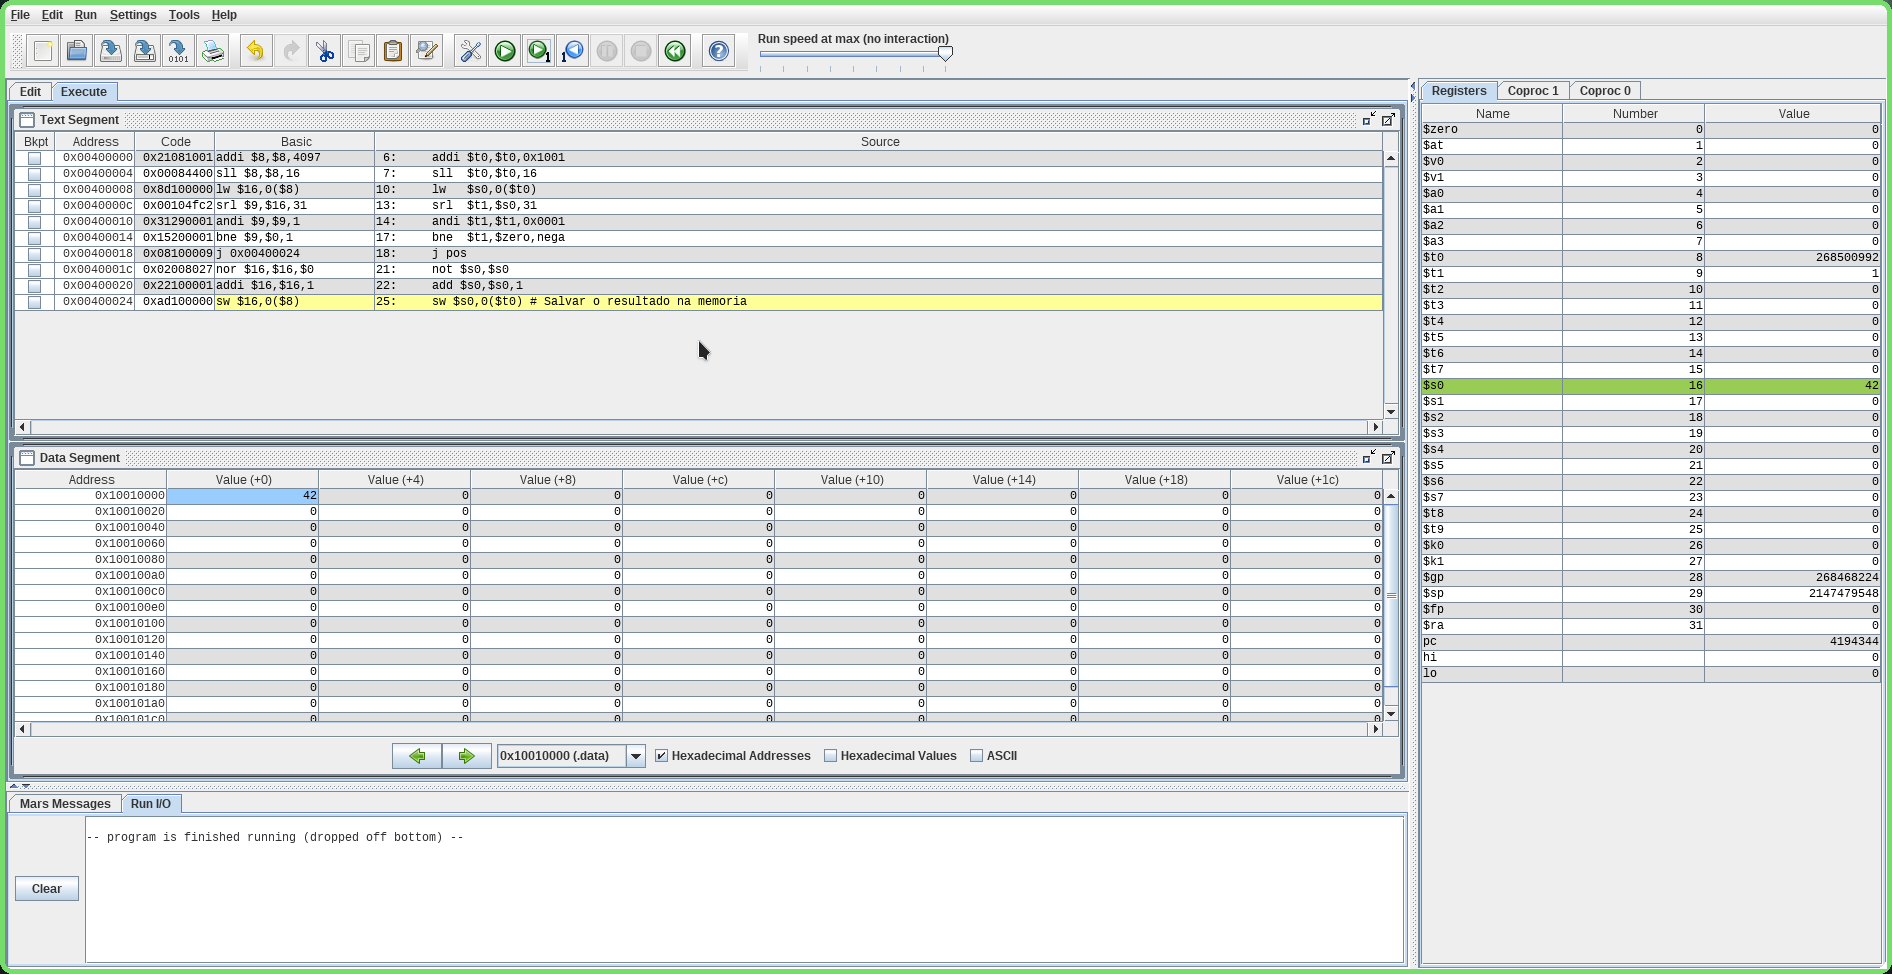
\includegraphics[width=1\textwidth]{programa13}
\end{figure}

\begin{figure}[!ht]
    \caption{Programa 14}
    \centering
    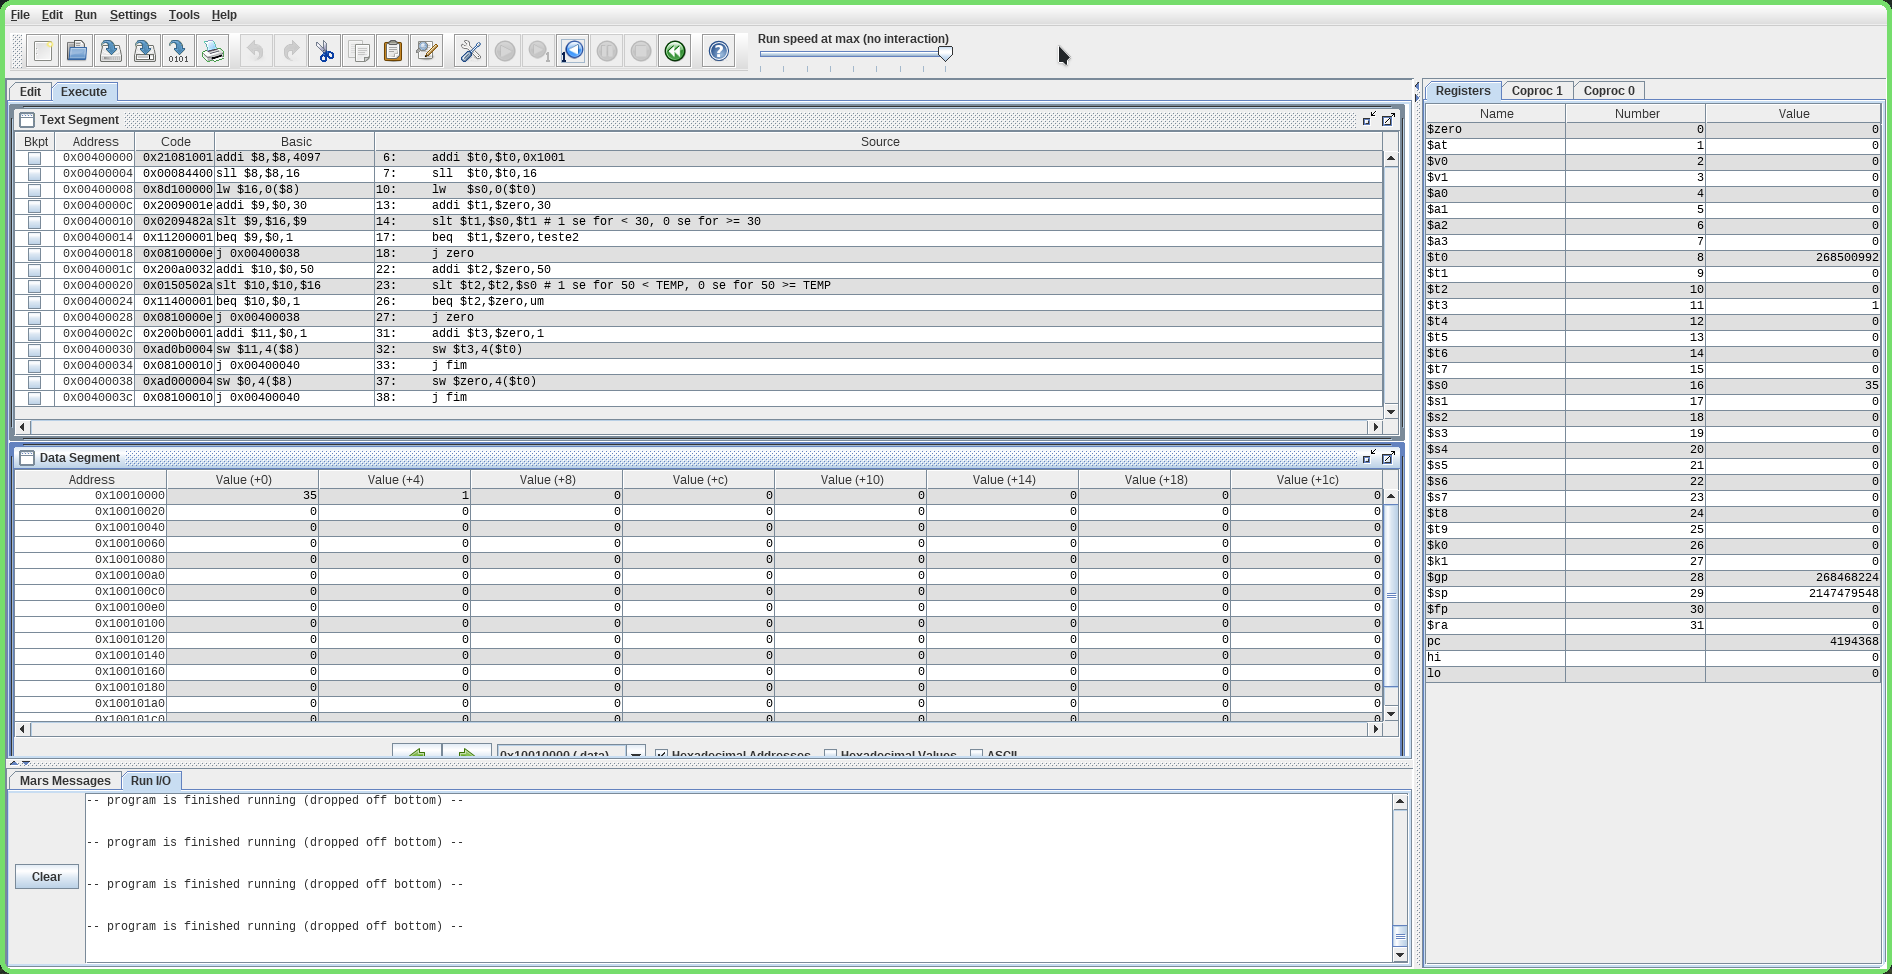
\includegraphics[width=1\textwidth]{programa14}
\end{figure} 

\begin{figure}[!ht]
    \caption{Programa 15}
    \centering
    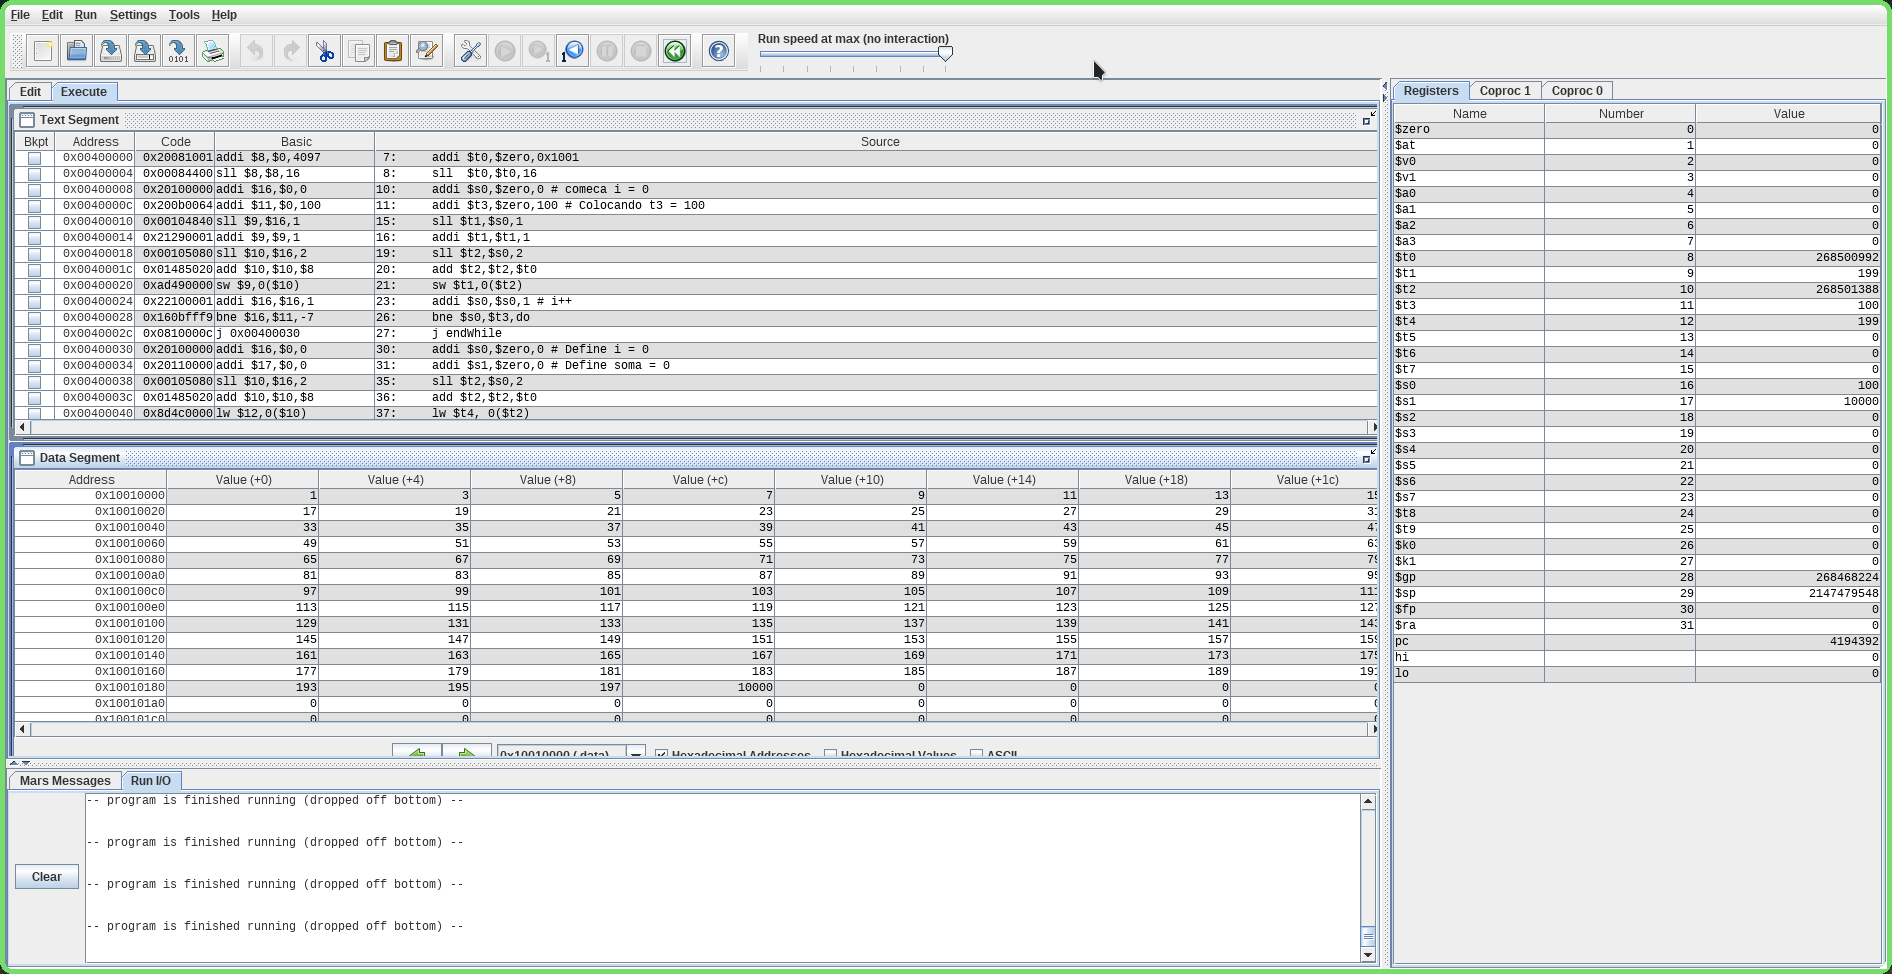
\includegraphics[width=1\textwidth]{programa15}
\end{figure}

\begin{figure}[!ht]
    \caption{Programa 16}
    \centering
    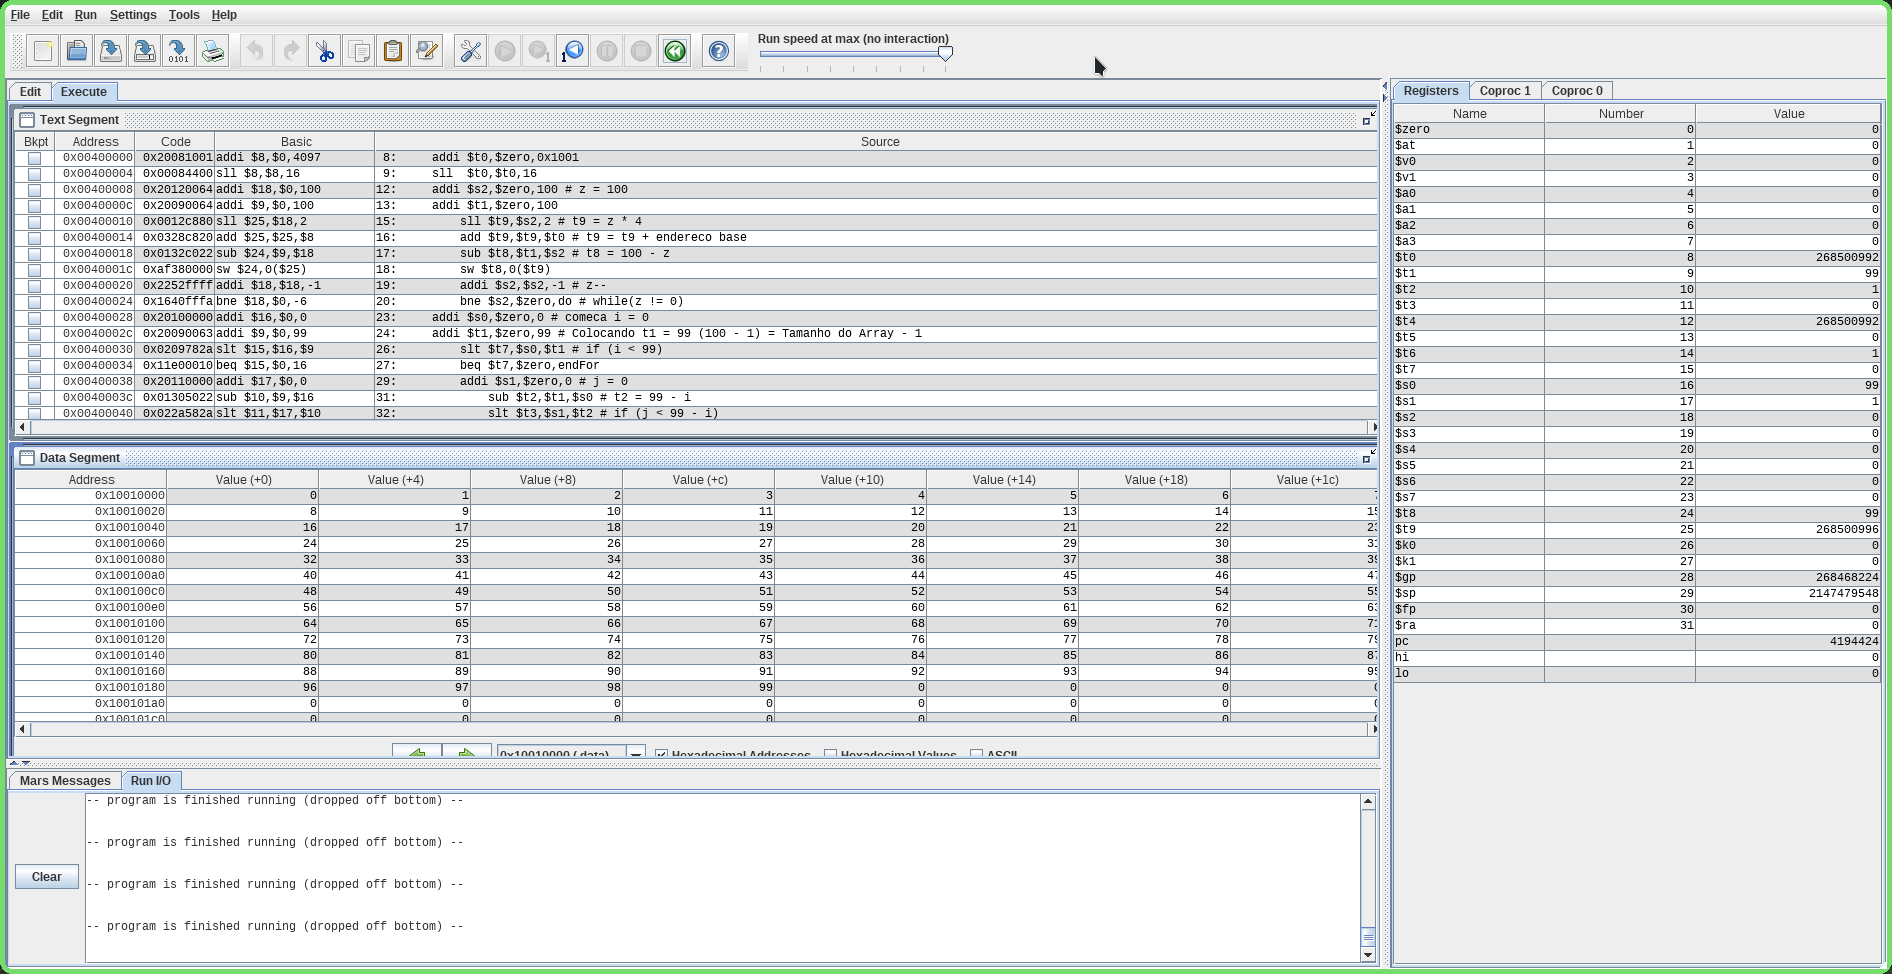
\includegraphics[width=1\textwidth]{programa16}
\end{figure} 

\begin{figure}[!ht]
    \caption{Programa 17}
    \centering
    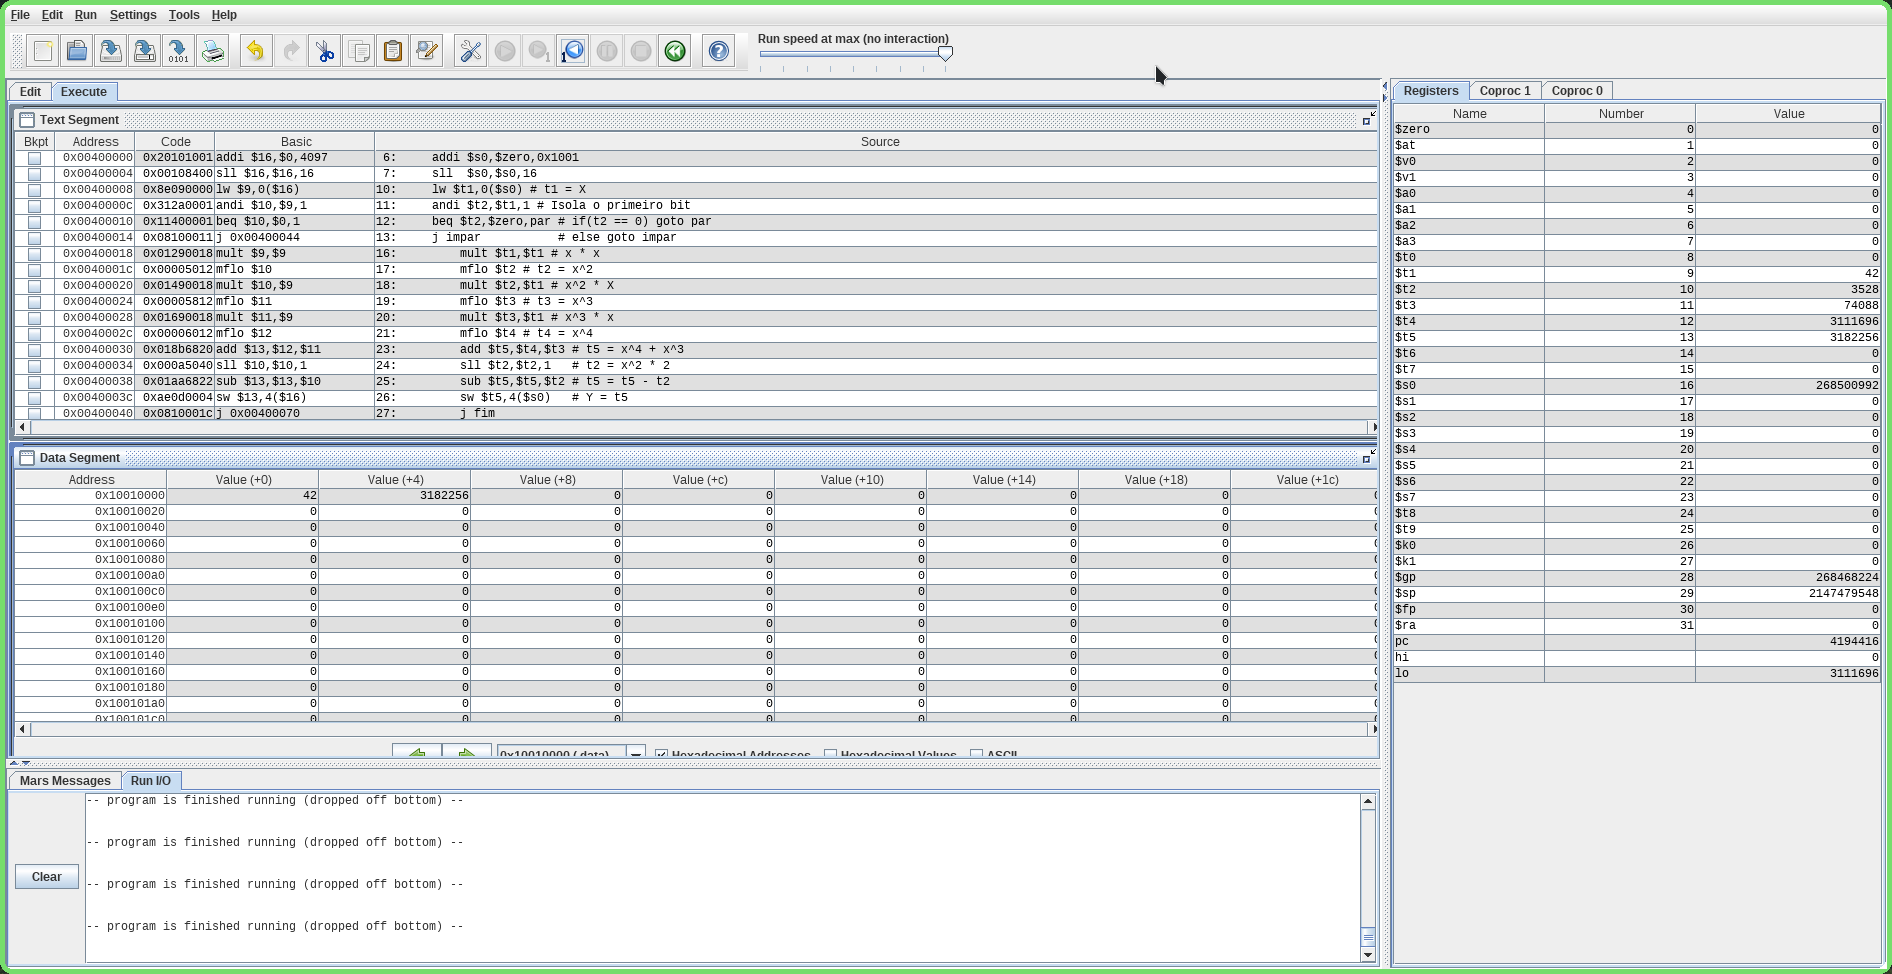
\includegraphics[width=1\textwidth]{programa17}
\end{figure}

\begin{figure}[!ht]
    \caption{Programa 18}
    \centering
    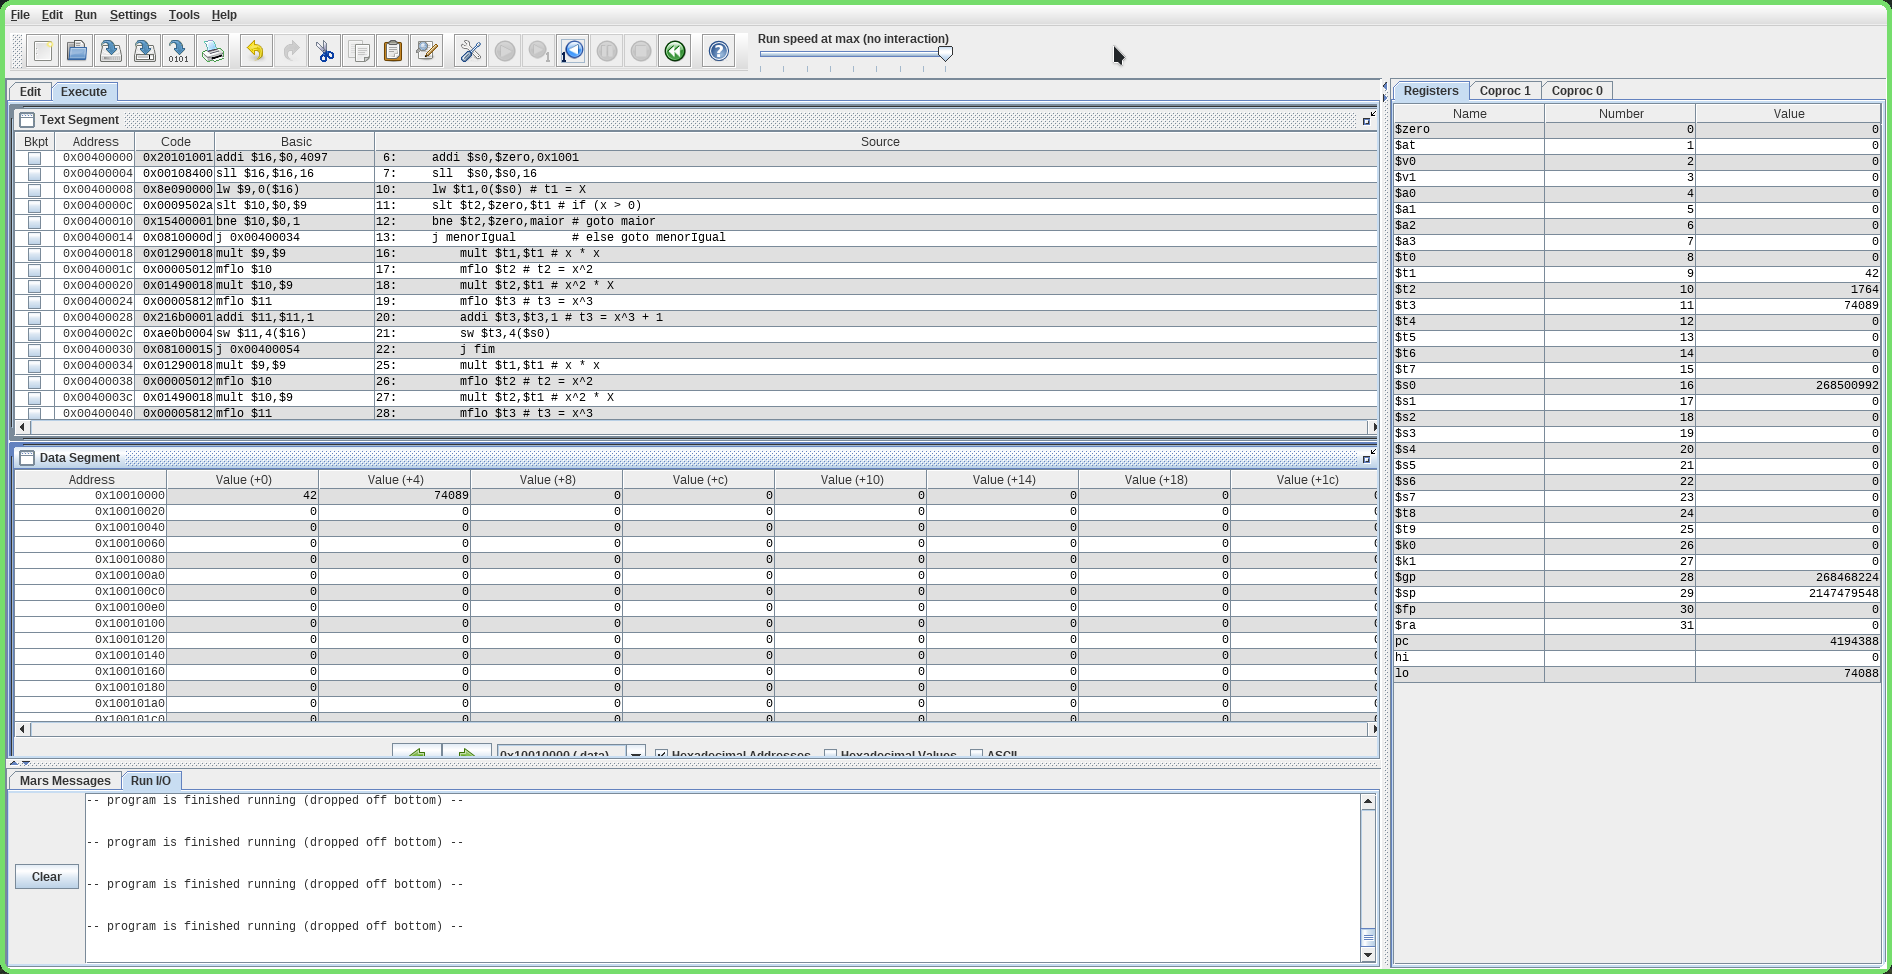
\includegraphics[width=1\textwidth]{programa18}
\end{figure}

\begin{figure}[!ht]
    \caption{Programa 19}
    \centering
    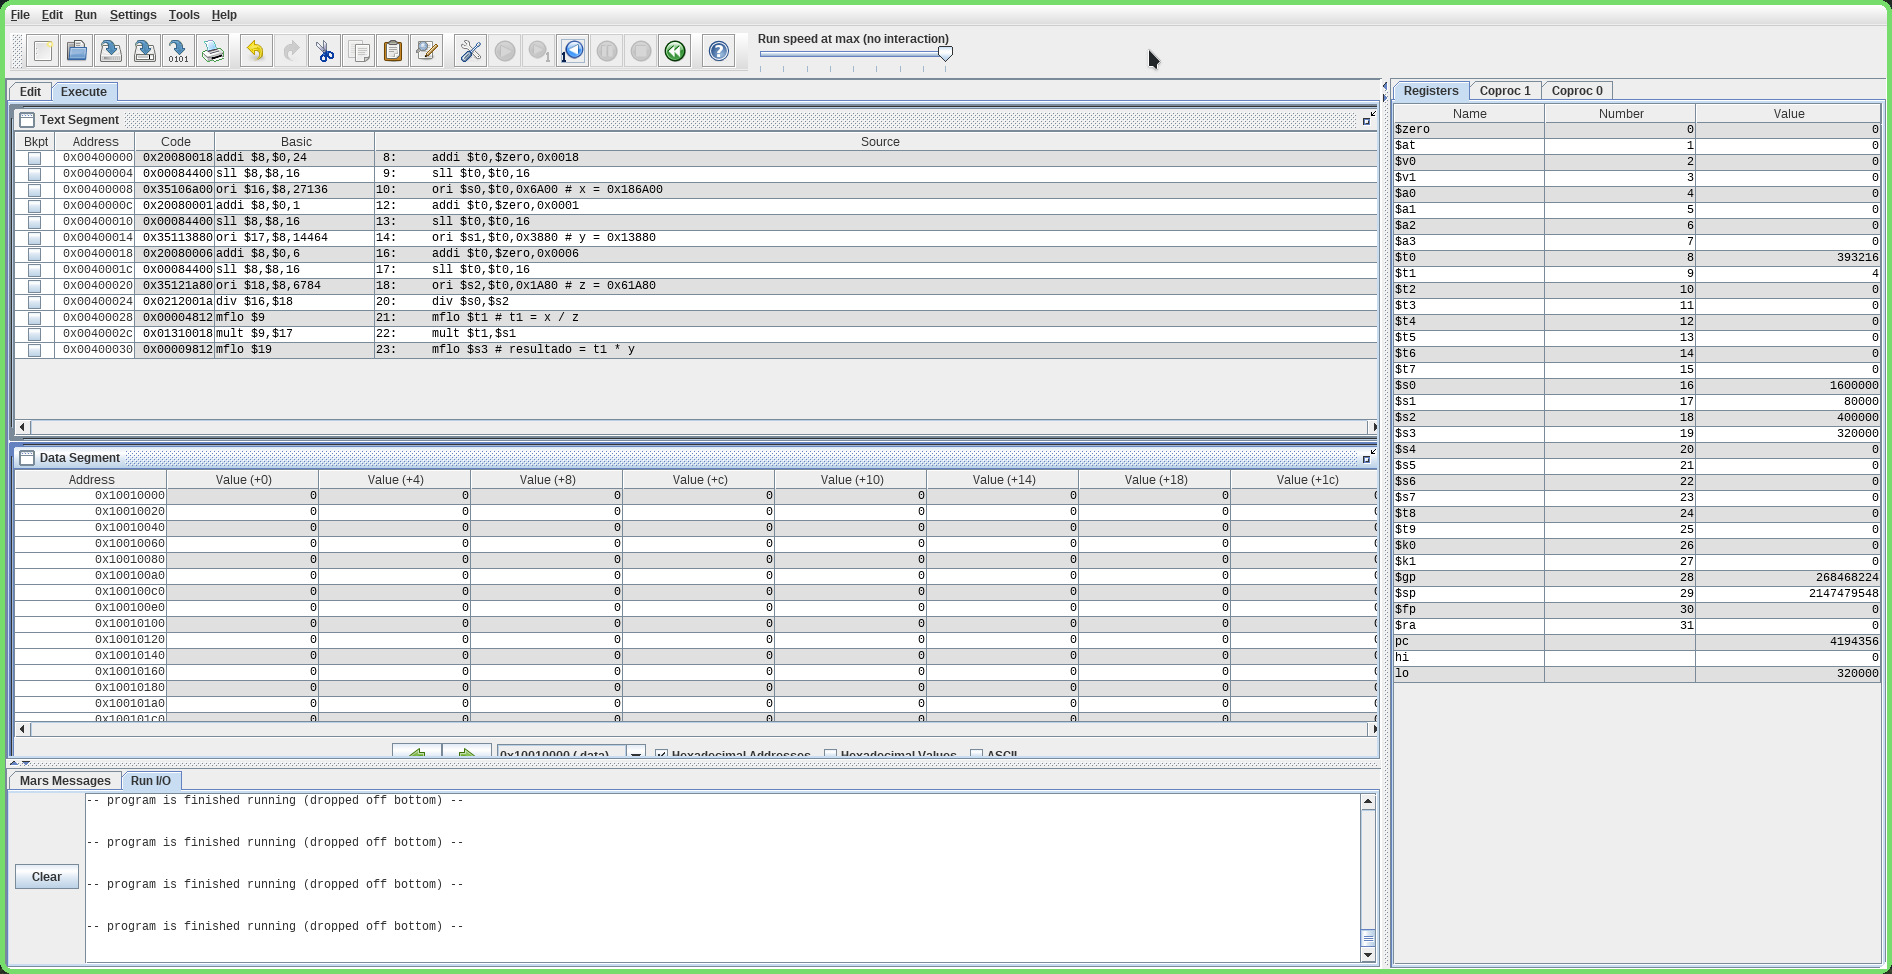
\includegraphics[width=1\textwidth]{programa19}
\end{figure}

\begin{figure}[!ht]
    \caption{Programa 20}
    \centering
    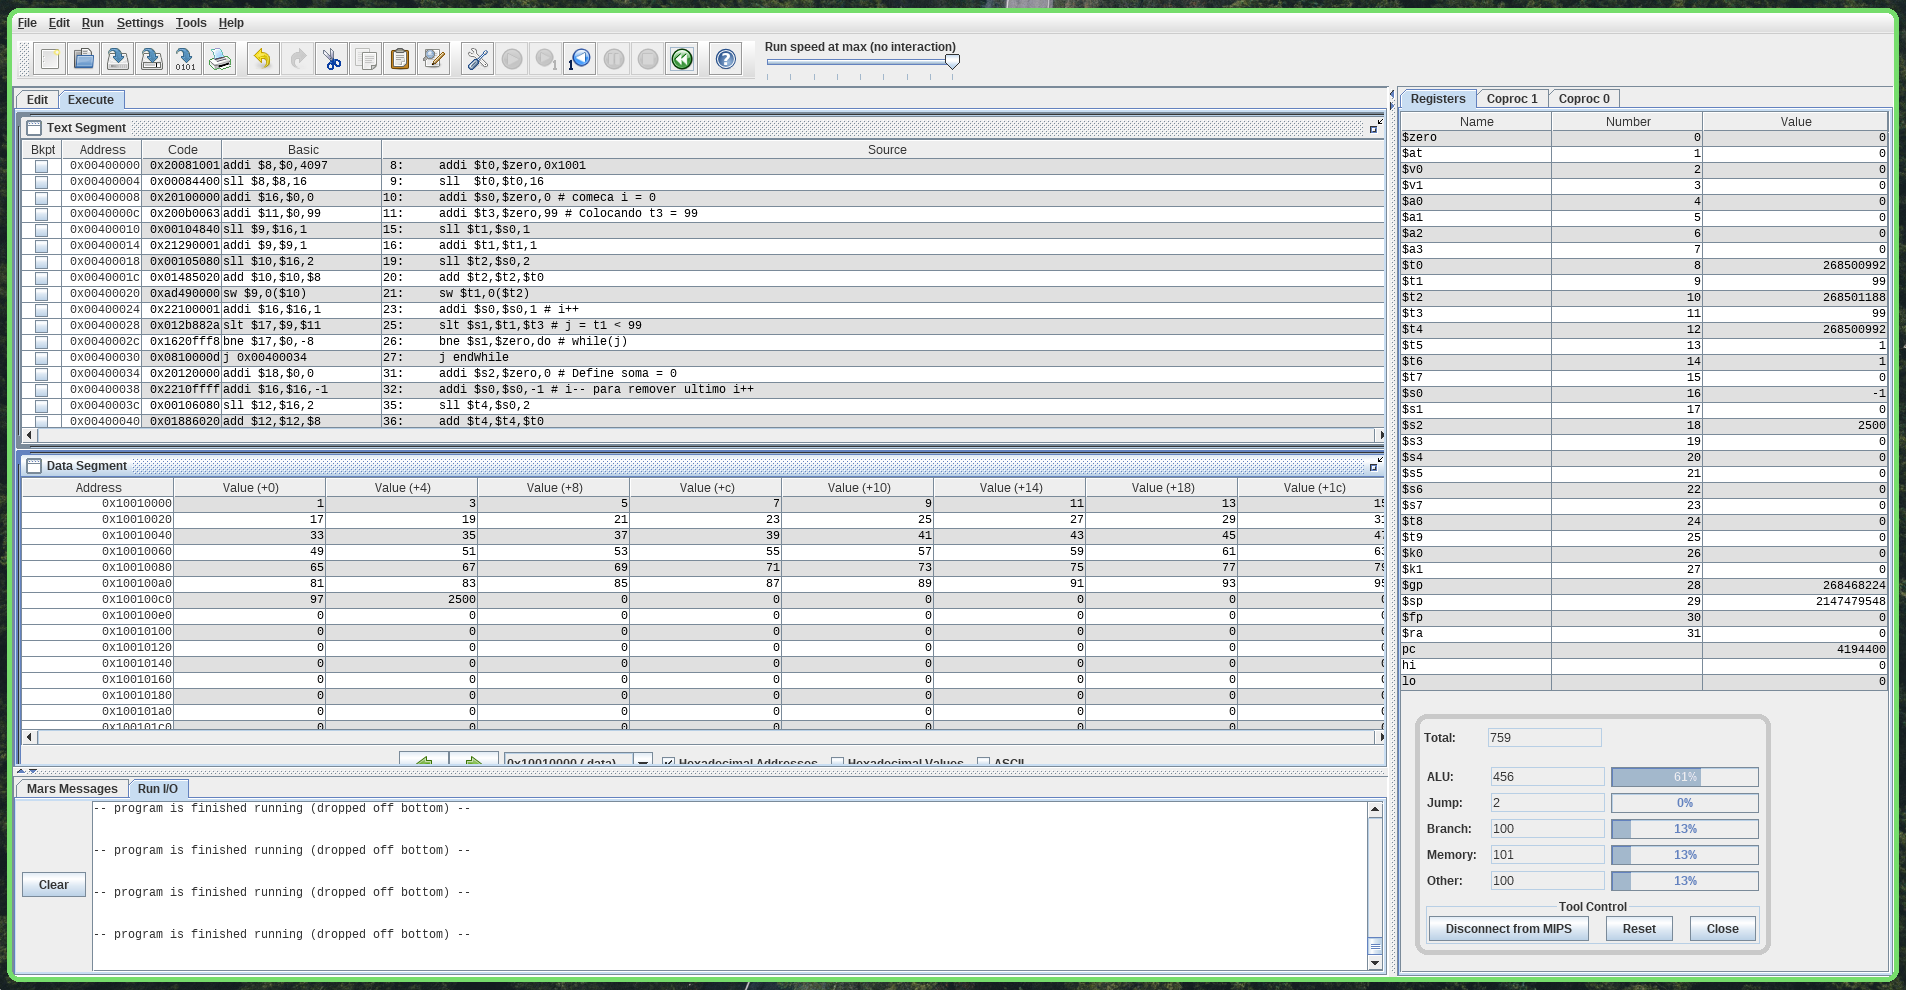
\includegraphics[width=1\textwidth]{programa20}
\end{figure}    

\begin{figure}[!ht]
    \caption{Programa 21}
    \centering
    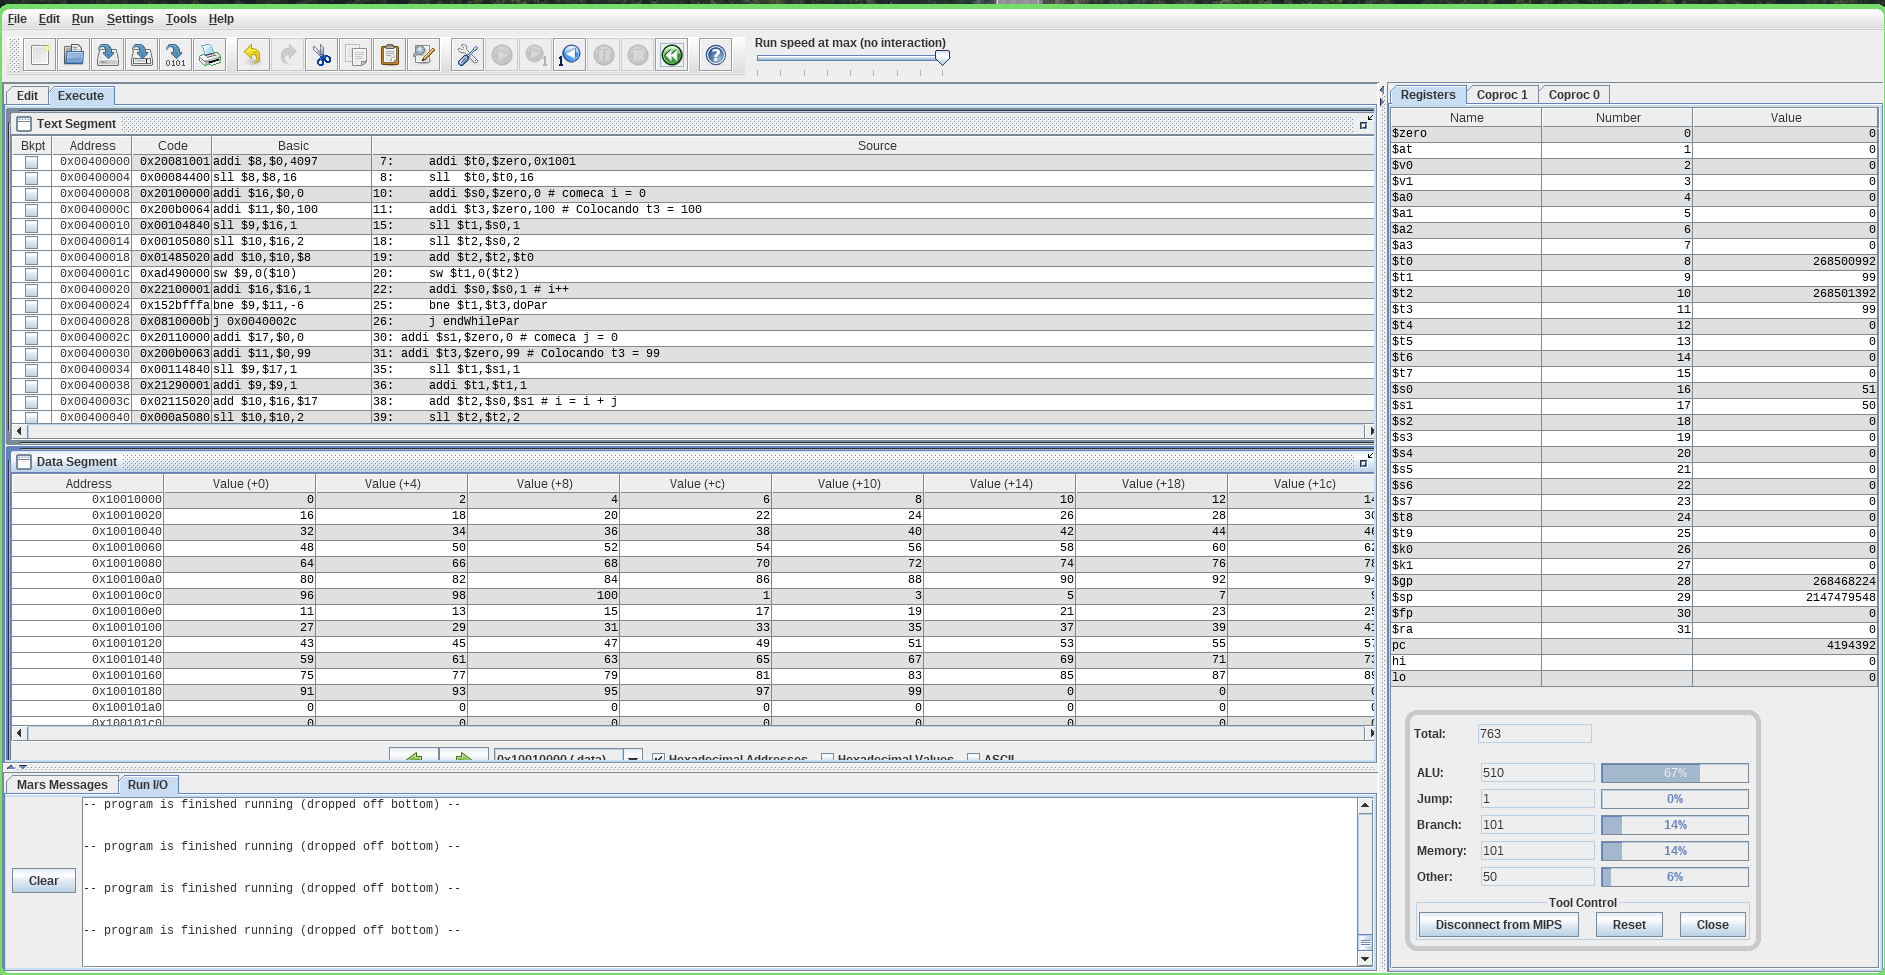
\includegraphics[width=1\textwidth]{programa21}
\end{figure}

\begin{figure}[!ht]
    \caption{Programa 22}
    \centering
    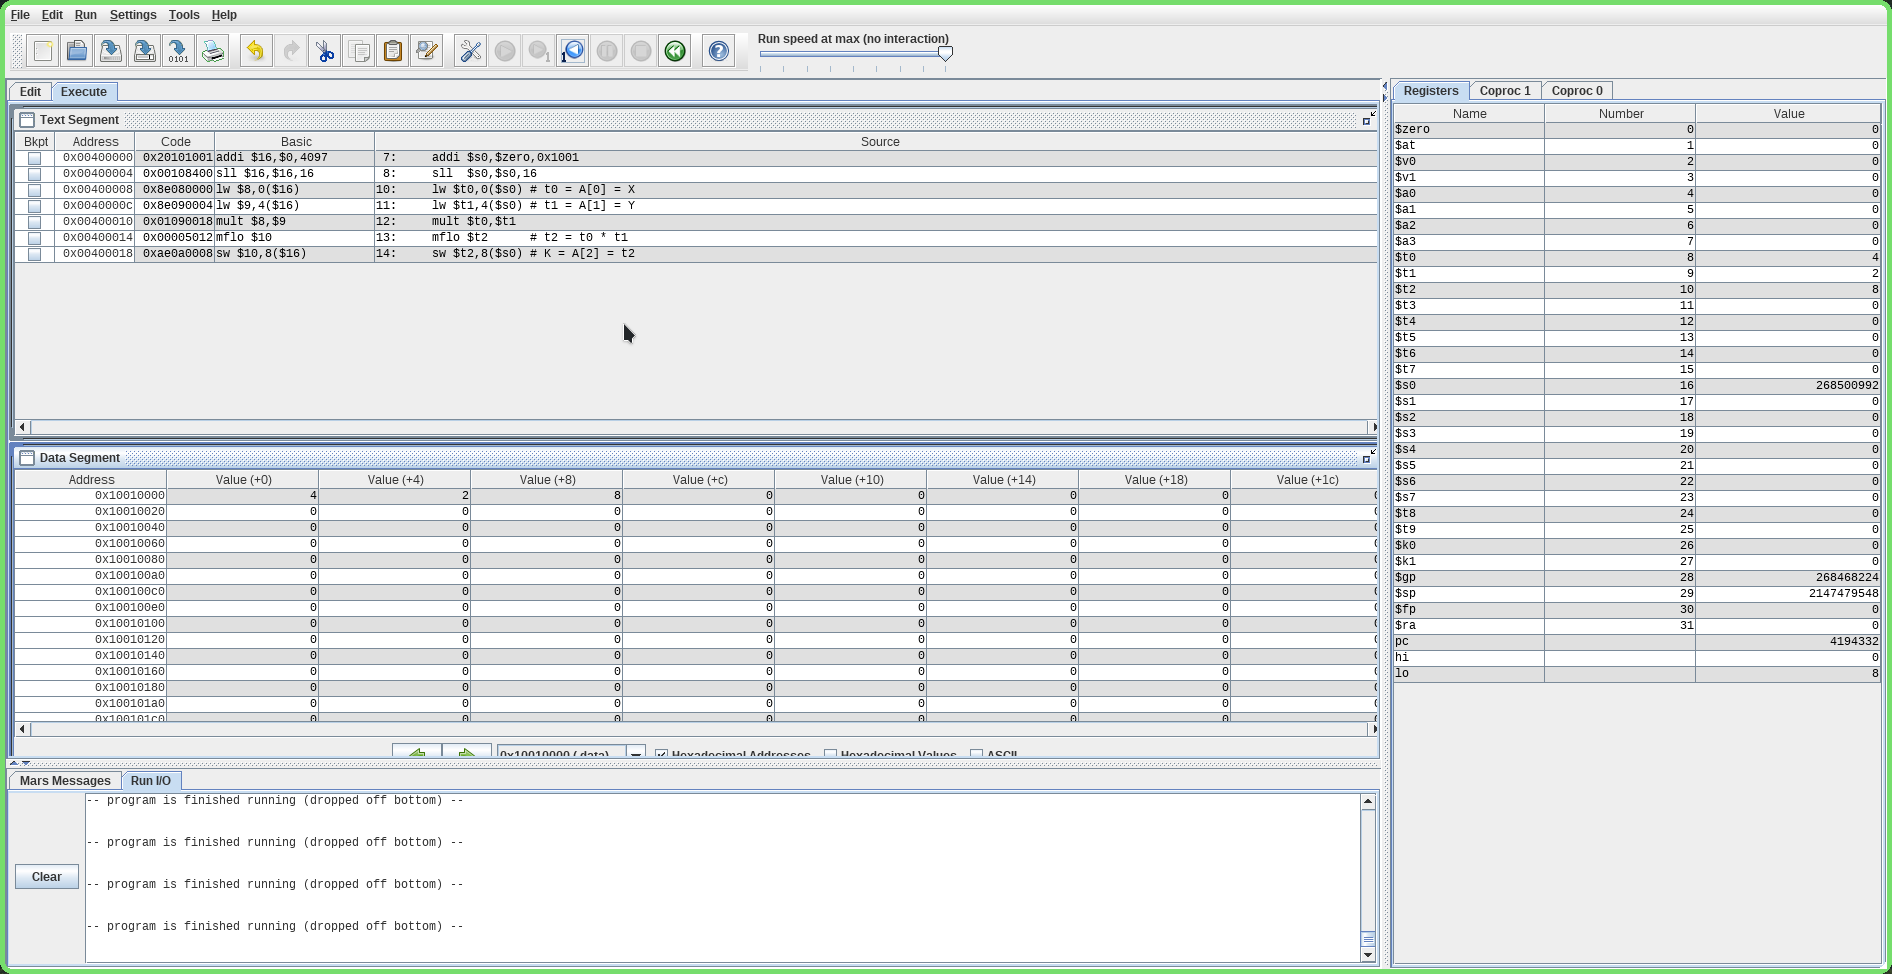
\includegraphics[width=1\textwidth]{programa22}
\end{figure} 
 
\begin{figure}[!ht]
    \caption{Programa 23}
    \centering
    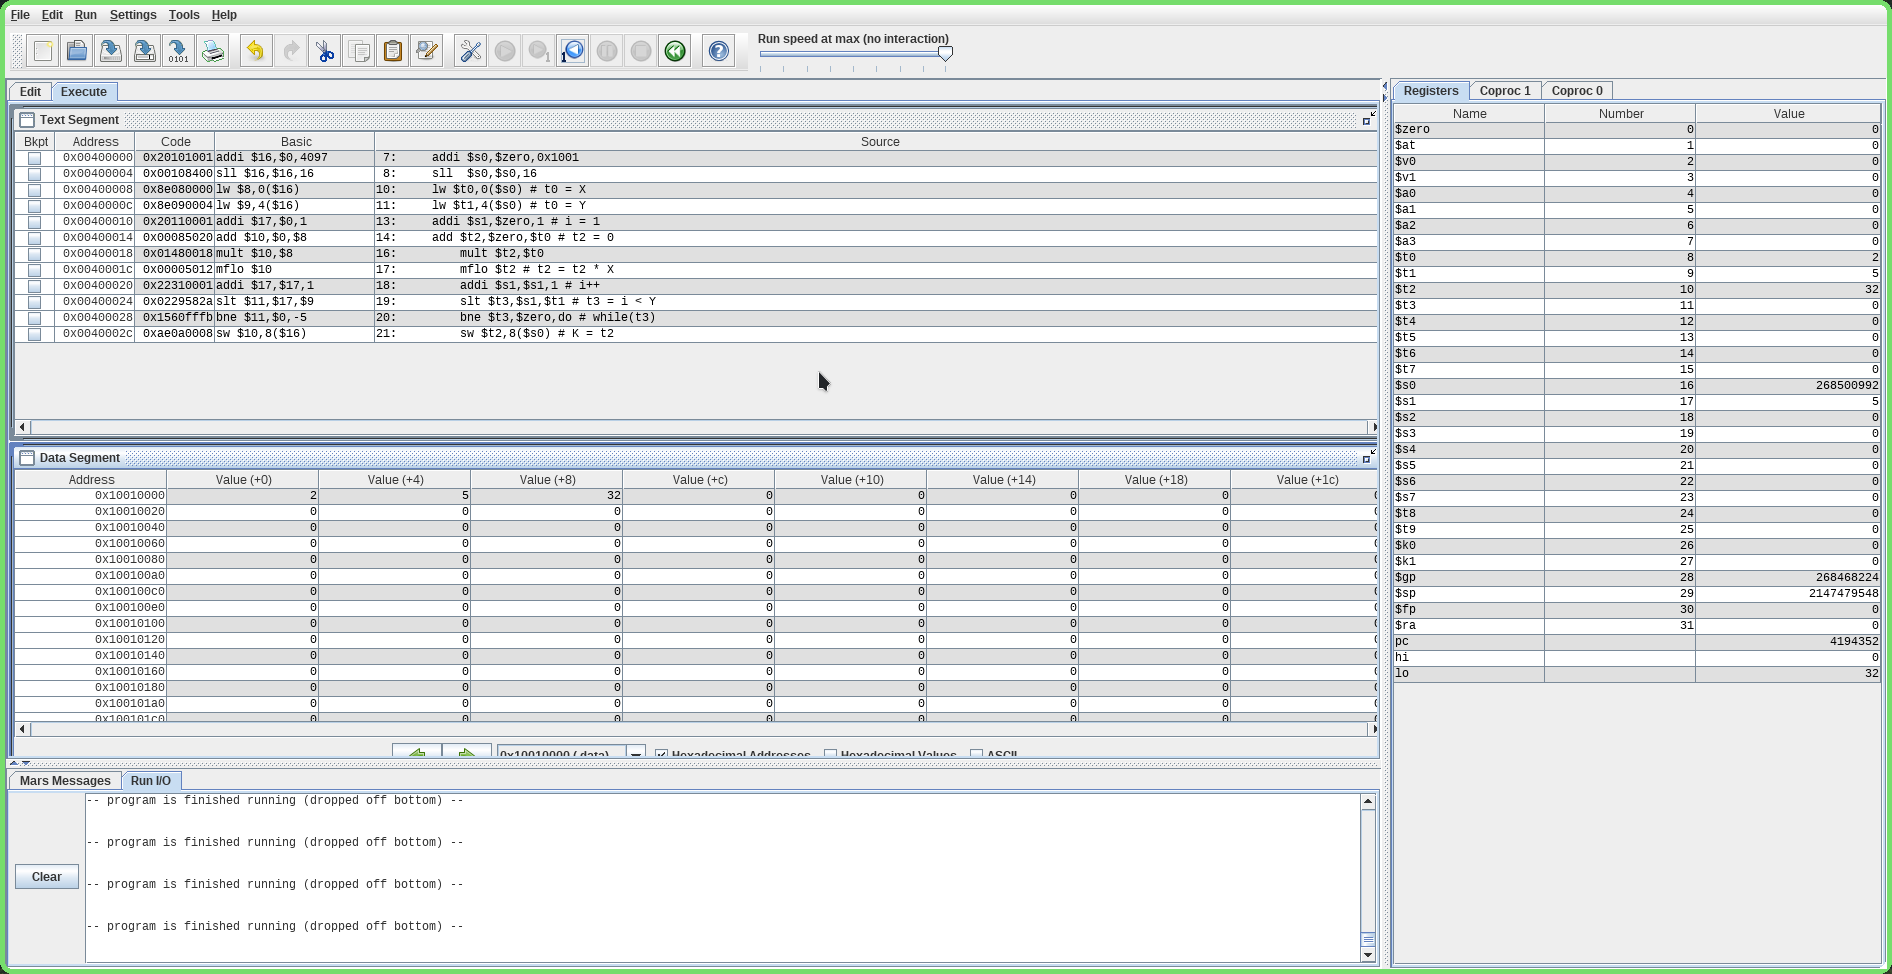
\includegraphics[width=1\textwidth]{programa23}
\end{figure} 

\end{document}
